\chapter{Ergodic Theorem}\label{chap32}

\begin{theorem*}
Let\pageoriginale $f:\mathbb{R}^{d}\to R$ be bounded and measurable
with $||f||_{\infty}\leq 1$. If $\phi$ is an invariant distribution
for the family $\{Q_{x}\}$, $x\in \mathbb{R}^{d}$ then 
$$
\lim\limits_{\substack{t_{1}\to \infty\\ 0\leq t_{2}-t_{1}\to
    \infty}}E^{Q_{x}}(f(X(t_{1}))f(X(t_{2})))=[\int f(y)\phi(y)dy]^{2}
$$
\end{theorem*}

\begin{proof}
\begin{align*}
& E^{Q_{x}}[(f(X(t_{1})f(X(t_{2}))]\\
& =E^{Q_{x}}(E^{Q_{x}}[f(X(t_{1}))f(X(t_{2}))|\mathscr{F}_{t_{1}}])\\
&
  =E^{Q_{x}}(f(X(t_{1}))(E^{Q_{x}}[f(X(t_{2}))|\mathscr{F}_{t_{1}}]))\\
& =E^{Q_{x}}(f(X(t_{1}))\int
  f(y)q(t_{2}-t_{1},X(t_{1}),y))dy),t_{2}>t_{1}\\
&\hspace{4cm} \text{(by Markov property),}\\
&= \int f(z)q(t_{1},x,z)dz\int
  f(y)q(t_{2}-t_{1},z,y)dy\tag{1}\label{chap32-eq1} 
\end{align*}
does any bounded an measurable $f$. By theorem of \S\ \ref{chap31},
$$
\sup\limits_{x\in K}|\int f(y)[q(t,x,y)-\phi(y)]dy|\to 0
$$
as $t\to +\infty$. We can therefore write \eqref{chap32-eq1} in the
form
\begin{align*}
& E^{Q_{x}}[(f(X(t_{1}))f(X(t_{2}))]=\\
&\qq =(\int f(z)q(t_{1},x,x)dz)\int f\phi+\int
  f(z)q(t_{1},x,z)A(t_{2}-t_{1},z)dz, 
\end{align*}
where $A(t_{2}-t_{1},z)$ converges to $0$ (uniformly on compact sets
as) $t_{2}-t_{1}\to +\infty$.

To\pageoriginale prove the theorem we have therefore only to show that
$$
\int f(z)q(t_{1},x,z)A(t_{2}-t_{1},z)dz\to 0
$$
as $t_{1}\to +\infty$ and $t_{2}-t_{1}\to \infty$ (because $\int
f(z)q(t_{1},x,z)dz\to \int f\phi$). Now
\begin{align*}
& |\int f(z)q(t_{1},x,z)A(t_{2}-t_{1},z)dz|\\
& \leq ||f||_{\infty}\int q(t_{1},x,z)|A(t_{2}-t_{1},z)|dz\\
& \leq \int q(t_{1},x,z)|A(t_{2}-t_{1},z)|dz\tag{2}\label{chap32-eq2}
\end{align*}

Let $K$ be any compact set, then
$$
\int\limits_{K}q(t_{1},x,z)dz=\int\chi_{K}q(t_{1},x,z)dz\to \int
\chi_{K}\phi(z)dz 
$$
at $t_{1}\to \infty$. Given $\epsilon>0$, let $K$ be compact so that
$$
|\int \chi_{{}_{K^{c}}}\phi(z)dz|\leq \epsilon;
$$
then $|\int \chi_{K^{c}}q(t_{1},x,z)dz|\leq 2\epsilon$ if $t_{1}\gg
0$. Using \eqref{chap32-eq2} we therefore get
\begin{align*}
& |\int f(z)q(t_{1}x,z)A(t_{2}-t_{1},z)dz|\\
& \leq
  \int\limits_{K}q(t_{1},x,z)|A(t_{2}-t_{1},z)|dz+\int\limits_{K^{c}}q(t_{1},x,z)|A(t_{2}-t_{1},z)|dz\\ 
&\leq
  \int\limits_{K}q(t_{1},x,z)|A(t_{2}-t_{1},z)|dz+2\int\limits_{K^{c}}q(t_{1},x,z)dz,\\
&\qq \text{since~ } |A(t_{2}-t_{1},z)|\leq 2,\\
&\leq
  \int\limits_{K}q(t_{1},x,z)|A(t_{2}-t_{1},z)|dz+2\epsilon,\text{~
    if~ } t_{1}\gg 0.
\end{align*}

The\pageoriginale theorem now follows from the fact that
$$
\lim\limits_{t_{2}-t_{1}\to \infty}\sup\limits_{z\in K}|A(t_{2}-t_{1},z)=0.
$$
\end{proof}

\noindent
{\bf Weak Ergodic Theorem.}
$$
\lim\limits_{t\to
  \infty}E^{Q_{x}}\left[|\frac{1}{t}\int\limits^{t}_{0}f(X(s))ds-f(x)\phi(x)dx|>\epsilon\right]=0. 
$$

\begin{proof}
\begin{align*}
& E^{Q_{x}}\left[|\frac{1}{t}\int\limits^{t}_{0}f(X(s))ds-\int
    f(x)\phi(x)dx|>\epsilon\right]\\ 
& \leq
  \frac{1}{\epsilon^{2}}E^{Q_{x}}\left[|\frac{1}{t}\int\limits^{t}_{0}f(X(s))ds-\int
    f(y)\phi(y)dy|^{2}\right], 
\end{align*}
by Tchebychev's inequality. We show that the right side $\to 0$ as
$t\to \infty$. Now
\begin{align*}
& E^{Q_{x}} \left[|\frac{1}{t}\int\limits^{t}_{0}f(X(s))ds-\int
  f\phi|^{2}\right]\\
&
  =E^{Q_{x}}[|\frac{1}{t^{2}}\int\limits^{t}_{0}\int\limits^{t}_{0}f(X(\sigma_{1}))f(X(\sigma_{2}))d\sigma_{1}\ d\sigma_{2}+(\int
    f\phi dy)\\
&\qq -2\frac{1}{t}\int\limits^{t}_{0}f(X(\sigma))d\sigma\int f\phi dy]
\end{align*}

Also
\begin{align*}
& \sup\limits_{x\in K}|E^{Q_{x}}[f(X(t))-\int f(y)\phi(y)dy]|\\
&\qq =\sup\limits_{x\in K}|\int q(t,x,y)f(y)dy-\int f(y)\phi(y)dy|\\
&\qq \leq ||f||_{\infty}\sup\limits_{x\in K}\int |q(t,x,y)-\phi(y)|dy;
\end{align*}
the\pageoriginale right hand side tends to $0$ as $t$ tends to
$+\infty$. Consider
{\fontsize{10pt}{12pt}\selectfont
\begin{align*}
&\qq |E^{Q_{x}}(\frac{1}{t}\int\limits^{t}_{0}f(X(\sigma))d\sigma-\int
f(y)\phi(y)dy)|\\
&= |E^{Q_{x}}\left(\frac{1}{t}\int\limits^{T}_{0}f(X(\sigma))d\sigma-\int
f(y)\phi(y)dy+\frac{1}{t}\int\limits^{t}_{0}f(X(\sigma))d\sigma\right),0\leq
T\leq t,\\
&\leq
\frac{1}{t}|\int\limits^{T}_{0}E^{Q_{x}}f(X(\sigma))d\sigma-T\int
f(y)\phi(y)dy|+\\
&\qq
+|E^{Q_{x}}\left(\frac{1}{t}\int\limits^{t}_{T}f(X(\sigma))d\sigma-\left(\frac{t-T}{t}\right)\int
f(y)\phi(y)dy\right)|. 
\end{align*}}

Given $\epsilon>0$ choose $T$ large so that
$$
|E^{Q_{x}}(f(X(\sigma))-\int f(y)\phi(y)dy|\leq \epsilon,\q (\sigma
\geq T).
$$

Then
\begin{align*}
& |E^{Q_{x}}\Big(\frac{1}{t}\int\limits^{t}_{0}f(X(\sigma))d\sigma-\int
f(y)\phi(y)dy|\leq\\
&\leq
|\frac{1}{t}\int\limits^{T}_{0}E^{Q_{x}}[f(X(\sigma))]-\frac{T}{t}\int
f(y)\phi(y)dy]|+\frac{t-T}{t}\epsilon\\
&\leq 2\epsilon 
\end{align*}
provided $t$ is large. Thus
$$
\lim\limits_{t\to
  +\infty}E^{Q_{x}}[\frac{1}{t}\int\limits^{t}_{0}f(X(\sigma))d\sigma]=\int
f\phi dy.
$$

To prove the result we have therefore only to show that
$$
\lim\limits_{t\to
  +\infty}E^{Q_{x}}\left(\frac{1}{t^{2}}\int\limits^{t}_{0}\int\limits^{t}_{0}f(X(\sigma_{1}))f(X(\sigma_{2}))d\sigma_{1}d\sigma_{2}\right)=\left[\int f(y)\phi(y)dy\right]^{2}
$$
\begin{figure}[H]
\centering
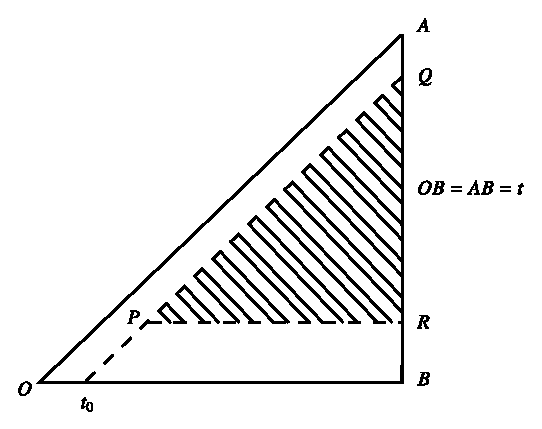
\includegraphics{figure/fig14.eps}
\end{figure}\pageoriginale

POR is the region $\sigma_{2}\geq t_{0}$, $\sigma_{1}-\sigma_{2}\geq
t_{0}$.

Let $I$
\begin{align*}
&
  =E^{Q_{x}}\left(\frac{1}{t}\int\limits^{t}_{0}\int\limits^{t}_{0}f(X(\sigma_{1}))f(X(\sigma_{2}))d\sigma_{1}d\sigma_{2}\right)-\left(\int
  f\phi dy\right)\\
&= \frac{2}{t^{2}}\int
  \left[E^{Q_{x}}(f(X(\sigma_{1}))f(X(\sigma_{2})))-\left(\int
    f(y)\phi(y)dy\right)^{2}\right]d\sigma_{1}d\sigma_{2}\\
&\q 0\leq \sigma_{2}\leq \sigma_{1}\leq t.
\end{align*}

Then
\begin{align*}
|I| &\leq \frac{2}{t^{2}}\int\limits_{\Delta
  PQR}|E^{Q_{x}}(f(X(\sigma_{1}))f(X(\sigma_{2})))-\left(\int
  f(y)\phi(y)dy\right)^{2}|d\sigma_{1}d\sigma_{2}\\
&\q +\frac{2}{t^{2}}\cdot 2||f||^{2}_{\infty}\q [\text{area of~ } OAB-
    \text{area of~ } PQR]
\end{align*}

By the Ergodic theorem the integrand of the first term on the right
can be made less than $\epsilon/2$ provided $t_{0}$ is large (see
diagram). Therefore
\begin{align*}
|I| &\leq \frac{\epsilon}{2}\cdot \frac{2}{t^{2}}\text{~ area of~ }PQR
+\frac{4}{t^{2}}||f||^{2}_{\infty}\left[\frac{t^{2}}{2}-\left(\frac{(t-2t_{0})}{2}\right)^{2}\right]\\ 
&\leq
\frac{\epsilon}{2}+\frac{2||f||^{2}_{\infty}}{t^{2}}[4tt_{0}-4t_{0}^{2}].\\
&<\epsilon 
\end{align*}\pageoriginale
if $t$ is large. This completes the proof of the theorem.
\end{proof}
